\documentclass[ngerman, fleqn, DIV=15, headinclude]{scrartcl}

\usepackage[color]{header}

\hypersetup{
    pdftitle=NetSec Sheet 4
}


\theoremstyle{definition}
\newtheorem{exercise}{Task}

\usepackage{tikz}
\usetikzlibrary{arrows.meta}

%\subject{}
\title{}
%\subtitle{}
\author{
    Timm Behner \\ \small{\href{mailto:behner@cs.uni-bonn.de}{behner@cs.uni-bonn.de}} \and
    Christopher Kannen \\ \small{\href{mailto:ckannen@uni-bonn.de}{ckannen@uni-bonn.de}}
}

\begin{document}

\maketitle

%\newpage
%\tableofcontents
%\newpage

\setcounter{exercise}{1}

\begin{exercise}
    The involved hosts are hellgate (10.0.0.1), white (10.0.0.5) and orange
    (10.0.0.10).
    \begin{figure}[H]
        \centering
        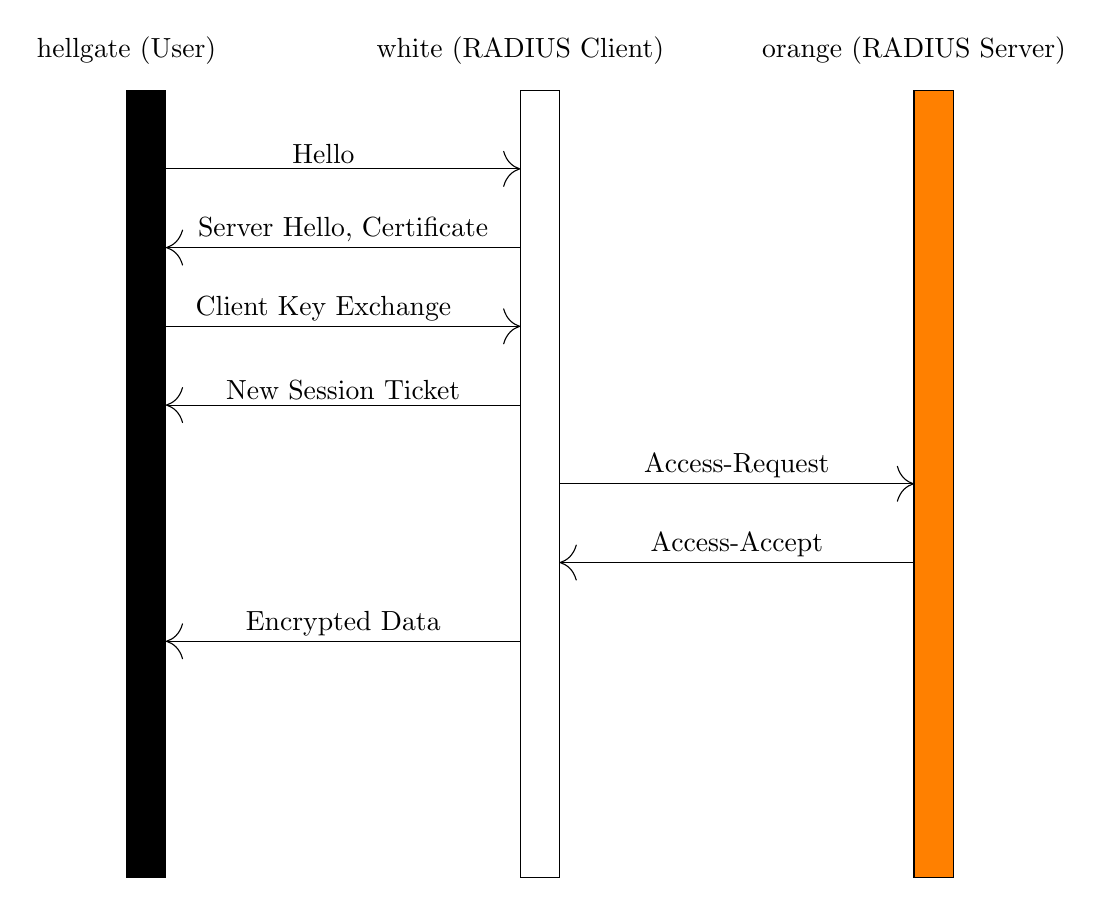
\begin{tikzpicture}
            \foreach \x/\text in {0/hellgate (User), 5/white (RADIUS Client),
            10/orange (RADIUS Server)}
            {
                \node at (\x,5.5) {\text};
            }
            \draw[fill=black] (0  ,-5) rectangle (0.5,5);
            \draw[fill=white] (5  ,-5) rectangle (5.5,5);
            \draw[fill=orange] (10,-5) rectangle (10.5,5);
            \draw[-{>[scale=2.5]}] (0,4) -- node[yshift=-5,label=Hello] {} (5,4);
            \draw[-{>[scale=2.5]}] (5,3) -- node[yshift=-5,label={Server Hello, Certificate}] {} (0.5,3);
            \draw[-{>[scale=2.5]}] (0,2) -- node[yshift=-5,label=Client Key Exchange] {} (5,2);
            \draw[-{>[scale=2.5]}] (5,1) -- node[yshift=-5,label={New Session Ticket}] {} (0.5,1);
            \draw[-{>[scale=2.5]}] (5.5,0) -- node[yshift=-5,label={Access-Request}] {} (10,0);
            \draw[-{>[scale=2.5]}] (10,-1) -- node[yshift=-5,label={Access-Accept}] {} (5.5,-1);
            \draw[-{>[scale=2.5]}] (5,-2) -- node[yshift=-5,label={Encrypted Data}] {} (0.5,-2);
        \end{tikzpicture}
    \end{figure}
\end{exercise}


\end{document}

% vim: spell spelllang=en tw=79
